\documentclass{article}

\usepackage{fancyhdr}
\usepackage{extramarks}
\usepackage{amsmath}
\usepackage{amsthm}
\usepackage{amsfonts}
\usepackage{tikz}
\usepackage[plain]{algorithm}
\usepackage{algpseudocode}
\usepackage[utf8]{inputenc}
\usepackage[T1]{fontenc}
\usepackage{natbib}

\usetikzlibrary{automata,positioning}

%
% Basic Document Settings
%

\topmargin=-0.45in
\evensidemargin=0in
\oddsidemargin=0in
\textwidth=6.5in
\textheight=9.0in
\headsep=0.25in

\linespread{1.1}

\pagestyle{fancy}
%\lhead{\hmwkAuthorName}
%\chead{\hmwkClass\ (\hmwkClassInstructor\ \hmwkClassTime): \hmwkTitle}
\lhead{\hmwkClass: \hmwkTitle}
\rhead{\hmwkAuthorName}
\lfoot{\lastxmark}
\cfoot{\thepage}

\renewcommand\headrulewidth{0.4pt}
\renewcommand\footrulewidth{0.4pt}

\setlength\parindent{0pt}
\setlength{\parskip}{1em}

%
% Create Problem Sections
%

\newcommand{\enterProblemHeader}[1]{
    \nobreak\extramarks{}{Problem \arabic{#1} continued on next page\ldots}\nobreak{}
    \nobreak\extramarks{Problem \arabic{#1} (continued)}{Problem \arabic{#1} continued on next page\ldots}\nobreak{}
}

\newcommand{\exitProblemHeader}[1]{
    \nobreak\extramarks{Problem \arabic{#1} (continued)}{Problem \arabic{#1} continued on next page\ldots}\nobreak{}
    \stepcounter{#1}
    \nobreak\extramarks{Problem \arabic{#1}}{}\nobreak{}
}

\setcounter{secnumdepth}{0}
\newcounter{partCounter}
\newcounter{homeworkProblemCounter}
\setcounter{homeworkProblemCounter}{1}
%\nobreak\extramarks{Problem \arabic{homeworkProblemCounter}}{}\nobreak{}

%
% Homework Problem Environment
%
% This environment takes an optional argument. When given, it will adjust the
% problem counter. This is useful for when the problems given for your
% assignment aren't sequential. See the last 3 problems of this template for an
% example.
%
\newenvironment{homeworkProblem}[1][-1]{
    \ifnum#1>0
        \setcounter{homeworkProblemCounter}{#1}
    \fi
    \section{Problem \arabic{homeworkProblemCounter}}
    \setcounter{partCounter}{1}
    \enterProblemHeader{homeworkProblemCounter}
}{
    \exitProblemHeader{homeworkProblemCounter}
}

%
% Homework Details
%   - Title
%   - Due date
%   - Class
%   - Section/Time
%   - Instructor
%   - Author
%

\newcommand{\hmwkTitle}{Description de projet}
\newcommand{\hmwkDueDate}{5 février, 2017}
\newcommand{\hmwkClass}{MTH8408}
\newcommand{\hmwkClassTime}{}
\newcommand{\hmwkClassInstructor}{Professeur Dominique Orban}
\newcommand{\hmwkAuthorName}{André Phu-Van Nguyen, 1525972}
\renewcommand{\refname}{Références}

%
% Title Page
%

\title{
    \vspace{2in}
    \textmd{\textbf{\hmwkClass:\ \hmwkTitle}}\\
    \normalsize\vspace{0.1in}\small{Remis\ pour\ le\ \hmwkDueDate\ }\\
    \vspace{0.1in}\large{\textit{\hmwkClassInstructor\ \hmwkClassTime}}
    \vspace{3in}
}

\author{\textbf{\hmwkAuthorName}}
\date{}

\renewcommand{\part}[1]{\textbf{\large Part \Alph{partCounter}}\stepcounter{partCounter}\\}

%
% Various Helper Commands
%

% Useful for algorithms
\newcommand{\alg}[1]{\textsc{\bfseries \footnotesize #1}}

% For derivatives
\newcommand{\deriv}[1]{\frac{\mathrm{d}}{\mathrm{d}x} (#1)}

% For partial derivatives
\newcommand{\pderiv}[2]{\frac{\partial}{\partial #1} (#2)}

% Integral dx
\newcommand{\dx}{\mathrm{d}x}

% Alias for the Solution section header
\newcommand{\solution}{\textbf{\large Solution}}
\newcommand{\norm}[1]{\left\lVert#1\right\rVert}

% Probability commands: Expectation, Variance, Covariance, Bias
\newcommand{\E}{\mathrm{E}}
\newcommand{\Var}{\mathrm{Var}}
\newcommand{\Cov}{\mathrm{Cov}}
\newcommand{\Bias}{\mathrm{Bias}}

\begin{document}

\maketitle

\pagebreak


\section{Développement du problème de génération de trajectoires}
Étant donné les sorties plates (les sorties d'un système différentiellement plat):
\begin{equation}
\sigma = [x, y, z, \psi]^T
\end{equation}
où $r = [x, y, z]^T$ est la position du centre de masse dans le système de coordonnées du monde et $\psi$ l'angle de lacet. Rappelons nous que dans un repère main droite centré sur un corps rigide, l'axe $x$ pointe vers l'avant, $y$ vers la gauche et $z$ vers le haut. Les angles de rotation autour de ces axes sont le roulis (\textit{roll}), tangage (\textit{pitch}) et lacet (\textit{yaw}) respectivement. À fin de garder le projet simple, nous ne considérons pas les angles de roulis et de tangage dans le problème mais nous savons qu'il est possible de le faire pour exécuter des manoeuvres accrobatiques tel que voler à travers une fenêtre inclinée.

\begin{figure}[h]
	\centering
	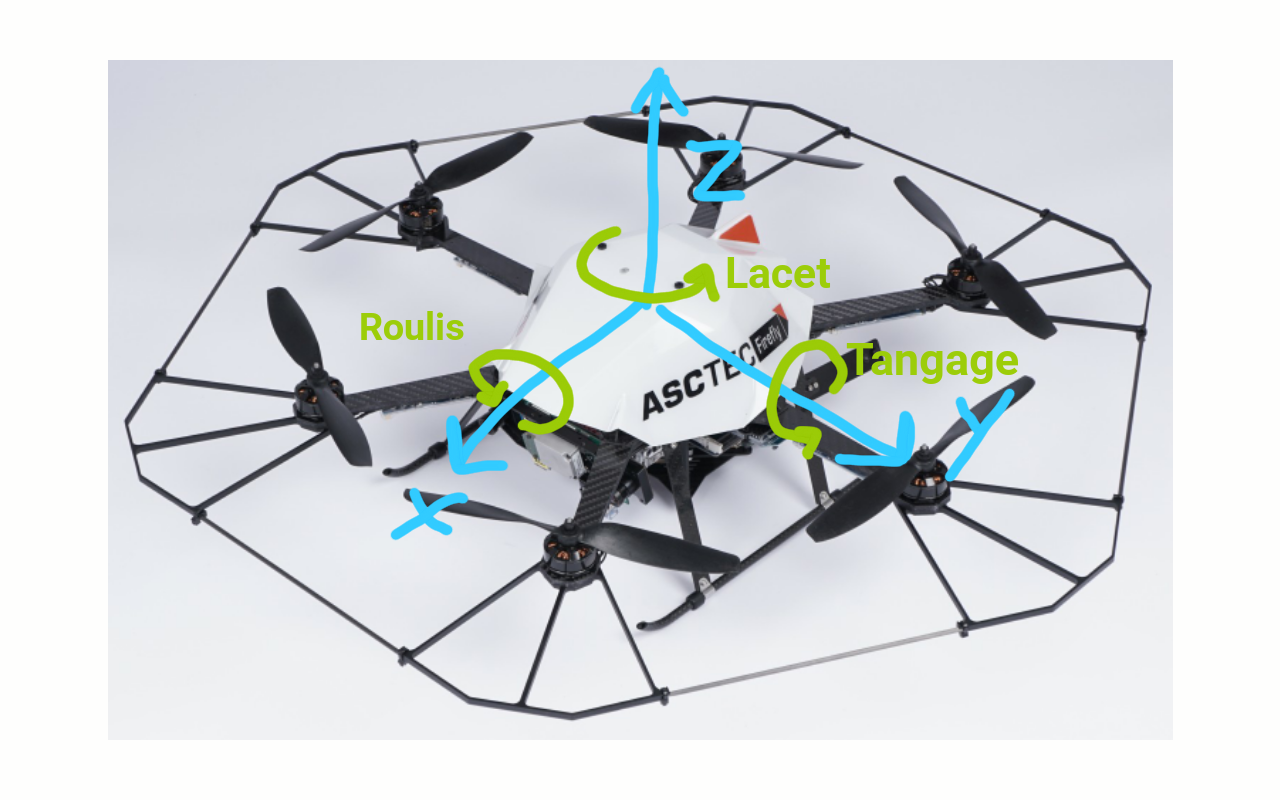
\includegraphics[width=0.5\textwidth]{fig/firefly.png}
	\caption{Systèmes de coordonnées d'un hexacoptère. L'angle de lacet est la rotation du véhicule autour de son axe Z, c'est-à-dire quand le véhicule tourne sur lui même.}
\end{figure}

Une trajectoire est définie comme étant une courbe lisse dans l'espace des sorties plates:
$$ \sigma(t) : [t_0, t_m] \rightarrow \mathbb{R}^3 \times SO(2)$$ 
où $t_0$ et $t_m$ sont les temps de début et de fin de la trajectoire, $m$ correspond au nombre d'intervales de temps entre chaque waypoint et $SO(2)$ est le groupe spécial orthogonal. Plus concrètement, une trajectoire est décrite par un polynôme défini par parties:
\begin{align}\label{eq:polynomial}
\sigma_T(t) =
\left\{
	\begin{array}{ll}
		\sum_{i=0}^n \sigma_{Ti1} t^i  & t_0 \leq t < t_1 \\
		\sum_{i=0}^n \sigma_{Ti2} t^i  & t_1 \leq t < t_2 \\
		... \\
		\sum_{i=0}^n \sigma_{Tim} t^i  & t_{m-1} \leq t < t_m \\
	\end{array}
\right.
\end{align}
où $n$ est l'ordre du polynôme, $m$ est encore le nombre d'intervales de temps et $\sigma_T (t) = [\boldsymbol{r}_T(t)^T, \psi_T(t)]^T$.

Étant donné que l'on veut optimiser la dérivée d'ordre $k_r = 4$ (le \textit{snap}) de la position au carré et la dérivée d'ordre $k_\psi = 2$ (accélération angulaire) de langle de lacet $\psi$ au carré, nous avons le problème d'optimisation:
\begin{align}\label{eq:opt}
\text{min} \int_{t_0}^{t_m} \mu_r \norm{\frac{d^4 \boldsymbol{r}_T}{dt^4}}^2 + \mu_\psi {\ddot{\psi}_T}^2 dt
\end{align}\begin{align*}
	\begin{array}{lll}
%		\text{sous contraintes} & \sigma_T(t_i) = \sigma_i & i = 0, \ldots, m\\
		\text{sous contraintes} & \boldsymbol{r}_T(t_i) = \boldsymbol{r}_i & i = 0, \ldots, m\\
		& \psi_T(ti)=\psi_i & i = 0, \ldots, m\\
		& \frac{d^p x_T}{dt^p}|_{t=t_j} = 0\ \text{ou libre,} & j = 0, m; p = 1, 2, 3, 4\\
		& \frac{d^p y_T}{dt^p}|_{t=t_j} = 0\ \text{ou libre,} & j = 0, m; p = 1, 2, 3, 4\\
		& \frac{d^p z_T}{dt^p}|_{t=t_j} = 0\ \text{ou libre,} & j = 0, m; p = 1, 2, 3, 4\\
		& \frac{d^p \psi_T}{dt^p}|_{t=t_j} = 0\ \text{ou libre,} & j = 0, m; p = 1, 2\\
	\end{array}
\end{align*}

où $\boldsymbol{r}_T = [x_T, y_T, z_T]^T$ et $r_i = [x_i, y_i, z_i]$. En d'autres mots, les $x_T$ 

\subsection{Structure du problème d'optimisation}

Le problème peut être formulé en tant que problème d'optimisation quadratique en réécrivant les constantes $\sigma_{T_{ij}} = [x_{T_{ij}}, y_{T_{ij}}, z_{T_{ij}}, \psi_{T_{ij}}]$ en un vecteur $c$ de dimension $4nm \times 1$ \footnote{$4$ degrés de liberté, $n$ coefficients car les polynômes sont d'ordre $n$ et $m$ polynômes $1$ pour chaque segment de trajectoire} avec les variables de décision $\{x_{T_{ij}}, y_{T_{ij}}, z_{T_{ij}}, \psi_{T_{ij}}\}$ pour avoir la forme standard:
\begin{align}\label{eq:opt_quad}
\text{min}\ \ \ c^THc+f^Tc
\end{align}\begin{align*}
	\begin{array}{ll}
	\text{s. c.} & Ac\leq b
	\end{array}
\end{align*}

Le vecteur $c$ est donc le vecteur contenant les coefficients des polynômes définissant la trajectoire avec en premier les coefficients du polynôme pour l'axe $x$, ensuite les coefficients du polynôme pour l'axe $y$, puis pour $z$ et enfin pour l'angle de lacet $\psi$.

\subsubsection{Structure du problème en une dimension}

Avant de construire la matrice $H$ nous devons développer les équations des polynômes représentant un segment de trajectoire i.e. la trajectoire entre deux waypoints. En réglant l'ordre du polynôme à $n = 6$ nous avons pour un axe de déplacement $p$ en 3D où $p = x$, $y$ ou $z$:
\begin{align*}
\boldsymbol{p} &= c_6 t^6 + c_5 t^5 + c_4 t^4 + c_3 t^3 + c_2 t^2+ c_1 t + c_0\\
\frac{d \boldsymbol{p}}{dt} &= 6 c_6 t^5 + 5 c_5 t^4 + 4 c_4 t^3 + 3 c_3 t^2 + 2c_2 t + c_1 + 0\\
\frac{d^2 \boldsymbol{p}}{dt^2} &= 
	(6\cdot 5) c_6 t^4 + (5 \cdot 4) c_5 t^3 + (4 \cdot 3) c_4 t^2 + (3 \cdot 2) c_3 t + 2c_2 + 0 + 0\\
\frac{d^3 \boldsymbol{p}}{dt^3} &= 
	(6\cdot 5\cdot 4) c_6 t^3 + (5 \cdot 4\cdot 3) c_5 t^2 + (4 \cdot 3\cdot 2 ) c_4 t + (3 \cdot 2) c_3 + 0 + 0 + 0\\
\frac{d^4 \boldsymbol{p}}{dt^4} &= 
	(6\cdot 5\cdot 4\cdot 3) c_6 t^2 + (5 \cdot 4\cdot 3\cdot 2) c_5 t + (4 \cdot 3\cdot 2 ) c_4 + 0 + 0 + 0 + 0\\
\end{align*}
Prendre la norme euclidienne au carré de la position est équivalent à prendre le carré de chaque polynôme. Donc pour un polynôme $p$ représentant un axe $x$, $y$ ou $z$ nous avons:
\begin{align}
\norm{\frac{d^4 \boldsymbol{p}}{dt^4}}^2 &= 
	\bigg((6\cdot 5\cdot 4\cdot 3) c_6 t^2 + (5 \cdot 4\cdot 3\cdot 2) c_5 t + (4 \cdot 3\cdot 2 ) c_4 \bigg)^2 \\
	&=	(6\cdot 5\cdot 4\cdot 3)^2 c_6^2 t^4 + (6\cdot 5\cdot 4\cdot 3)(5 \cdot 4\cdot 3\cdot 2) c_6 c_5 t^3 + (6 \cdot 5 \cdot 4\cdot 3)(4\cdot 3\cdot 2)c_6 c_4 t^2 \nonumber\\
	&	+ (5 \cdot 4\cdot 3\cdot 2)^2 c_5^2 t^2 + (6\cdot 5\cdot 4\cdot 3)(5 \cdot 4\cdot 3\cdot 2) c_6 c_5 t^3 + (5 \cdot 4\cdot 3\cdot 2)(4\cdot 3\cdot 2)c_5 c_4 t \nonumber\\
	&	+ (4\cdot 3\cdot 2)^2 c_4^2 + (6 \cdot 5 \cdot 4\cdot 3)(4\cdot 3\cdot 2)c_6 c_4 t^2 + (5 \cdot 4\cdot 3\cdot 2)(4\cdot 3\cdot 2)c_5 c_4 t \nonumber\\
	& = (6\cdot 5\cdot 4\cdot 3)^2 c_6^2 t^4 + 2(6\cdot 5\cdot 4\cdot 3)(5 \cdot 4\cdot 3\cdot 2) c_6 c_5 t^3 + 2(6 \cdot 5 \cdot 4\cdot 3)(4\cdot 3\cdot 2)c_6 c_4 t^2 \nonumber\\
	&	+ (5 \cdot 4\cdot 3\cdot 2)^2 c_5^2 t^2 + 2 (5 \cdot 4\cdot 3\cdot 2)(4\cdot 3\cdot 2)c_5 c_4 t \nonumber\\
	&	+ (4\cdot 3\cdot 2)^2 c_4^2 \nonumber
\end{align}

Ensuite, pour un waypoint $j$ nous avons le temps de départ $t_j$ et le temps d'arrivée au prochain waypoint $t_{j+1}$, nous pouvons écrire le résultat de l'intégrale:
\begin{align}\label{eq:polynome_integre}
\int_{t_j}^{t_{j+1}} \norm{\frac{d^4 \boldsymbol{p}}{dt^4}}^2 dt
	& = \int_{t_j}^{t_{j+1}} (6\cdot 5\cdot 4\cdot 3)^2 c_6^2 t^4 + 2(6\cdot 5\cdot 4\cdot 3)(5 \cdot 4\cdot 3\cdot 2) c_6 c_5 t^3 \\
	&	+ 2(6 \cdot 5 \cdot 4\cdot 3)(4\cdot 3\cdot 2)c_6 c_4 t^2 + (5 \cdot 4\cdot 3\cdot 2)^2 c_5^2 t^2 + 2(5 \cdot 4\cdot 3\cdot 2)(4\cdot 3\cdot 2)c_5 c_4 t \nonumber \\
	&	+ (4\cdot 3\cdot 2)^2 c_4^2 \ dt\nonumber \\
%	&= (6\cdot 5\cdot 4\cdot 3)^2 c_6^2 \frac{1}{4} t^3 \Big|_{t_j}^{t_{j+1}} + 2(6\cdot 5\cdot 4\cdot 3)(5 \cdot 4\cdot 3\cdot 2) c_6 c_5 \frac{1}{3} t^2\Big|_{t_j}^{t_{j+1}}\nonumber \\
%	&	+ 2(6\cdot 5\cdot 4\cdot 3)(4\cdot 3\cdot 2) c_6 c_4 \frac{1}{2} t\Big|_{t_j}^{t_{j+1}}
%		+ (5 \cdot 4\cdot 3\cdot 2)^2 c_5^2 \frac{1}{2} t\Big|_{t_j}^{t_{j+1}} \nonumber \\
	&=	360^2 c_6^2 \frac{1}{4} t^4 \Big|_{t_j}^{t_{j+1}}
		+ 2 \cdot 360 \cdot 120 c_6 c_5 \frac{1}{3} t^3\Big|_{t_j}^{t_{j+1}}
		+ 2 \cdot 360 \cdot 24 c_6 c_4 \frac{1}{2} t^2\Big|_{t_j}^{t_{j+1}} \nonumber \\
	&	+ 120^2 c_5^2 \frac{1}{3} t^3\Big|_{t_j}^{t_{j+1}} + 2 \cdot 120 \cdot 24 c_5 c_4 \frac{1}{2}t^2 \Big|_{t_j}{t_{j+1}} \nonumber \\
	&	+ 24^2 c_4^2 t\Big|_{t_j}^{t_{j+1}} \nonumber
\end{align}


Avec le résultat en (\ref{eq:polynome_integre}) on peut maintenant poser une partie de la matrice $H$ de (\ref{eq:opt_quad}).

Tel qu'indiqué précédemment, le vecteur $c$ contient tous les coefficients de tous les polynômes de chaque segment de la trajectoire et de chaque degré de liberté. La partie de $c$ correspondant à un axe $p$ est donc $[c_6,\ c_5,\ c_4,\ c_3,\ c_2,\ c_1,\ c_0]^T$. Par conséquent, nous pouvons déduire la matrice $H_pj$ correspondante pour un waypoint $j$
\begin{align*}
H_p =
\begin{bmatrix}
    360^2 c_6^2 \frac{1}{4} t^3 \Big|_{t_j}^{t_{j+1}}
    	& 2 \cdot 360 \cdot 120 c_6 c_5 \frac{1}{3} t^2\Big|_{t_j}^{t_{j+1}}
    	& 2 \cdot 360 \cdot 24 c_6 c_4 \frac{1}{2} t\Big|_{t_j}^{t_{j+1}}
    	& 0
    	& 0
    	& 0
    	& 0 \\
    2 \cdot 360 \cdot 120 c_6 c_5 \frac{1}{3} t^2\Big|_{t_j}^{t_{j+1}}
    	& 120^2 c_5^2 \frac{1}{3} t^3\Big|_{t_j}^{t_{j+1}} 
    	& 2 \cdot 120 \cdot 24 c_5 c_4 \frac{1}{2}t^2 \Big|_{t_j}^{t_{j+1}} & 0 & 0 & 0 & 0\\
	2 \cdot 360 \cdot 24 c_6 c_4 \frac{1}{2} t\Big|_{t_j}^{t_{j+1}}
		& 2 \cdot 120 \cdot 24 c_5 c_4 \frac{1}{2}t^2 \Big|_{t_j}^{t_{j+1}} 
		& 24^2 c_4^2 t\Big|_{t_j}^{t_{j+1}} & 0 & 0 & 0 & 0 \\
    0 & 0 & 0 & 0 & 0 & 0 & 0 \\
    0 & 0 & 0 & 0 & 0 & 0 & 0 \\
    0 & 0 & 0 & 0 & 0 & 0 & 0 \\
    0 & 0 & 0 & 0 & 0 & 0 & 0 \\
\end{bmatrix}
\end{align*}

Suivant un raisonnement similaire, nous pouvons calculer $H_\psi$.

\subsubsection{Structure de l'Hessienne finale}

Une fois le développement précédent fait, nous pouvons concaténer en diagonale les quatres matrices $H_{xj}$, $H_{yj}$, $H_{zj}$, et $H_{\psi j}$ pour un waypoint $j$, pour chaque waypoint jusqu'au dernier waypoint $j=m$ pour former $H$ de (\ref{eq:opt_quad}).

\begin{align}
H=
\begin{bmatrix}
	H_{xj} \\
	&	H_{yj} \\
	&	&		H_{zj} \\
	&	&		&		H_{\psi j} \\
	&	&		&		&			\ddots \\
	&	&		&		&			&		H_{xm} \\
	&	&		&		&			&		&		H_{ym} \\
	&	&		&		&			&		&		&		H_{zm} \\
	&	&		&		&			&		&		&		&		H_{\psi m} \\
\end{bmatrix}
\end{align}

De plus, par le développement précédent en (\ref{eq:polynome_integre}), nous pouvons voir que le terme linéaire $f^Tc$ de (\ref{eq:opt_quad}) est nul.

%\section{Description de la problématique choisie}
%Pour ce projet nous avons choisi de reproduire la méthodologie et les résultats de l'article scientifique intitulé \textit{Minimum Snap Trajectory Generation and Control for Quadrotors} par Daniel Mellinger et Vijay Kumar. Dans cet article, les auteurs avaient entres autres l'objectif de générer des trajectoires qui prennent avantage de la dynamique des quadricoptères plutôt que de voir la dynamique en tant que contrainte sur le système \cite{Mellinger2011}. 
%
%Lors du suivi d'une trajectoire, une solution triviale est souvent utilisée qui consiste en l'interpolation en ligne droite entre chaque point de cheminement aussi nommé \textit{waypoint}. Ceci est inneficace car la courbure infinie à chaque waypoint oblige le quadricoptère à s'arrêter avant de passer au prochain waypoint. Mellinger propose donc de modéliser une trajectoire optimale par un polynôme défini par parties entièrement lisse à travers les différents waypoints tout en satisfaisant des contraintes sur les vitesses et accélérations possibles du véhicule. Ce problème est résolu en le reécrivant en problème d'optimisation quadratique.
%
%Tout dabord Mellinger démontre que la dynamique d'un quadricoptère a la propriété dêtre différentiellement plat. C'est-à-dire que les états et les entrées peuvent être exprimées par quatre sorties plates et leurs dérivées. Nous avons donc le vecteur de sorties plates
%$$\sigma = [x, y, z, \psi]^T$$
%où $r = [x, y, z]^T$ est la position du centre de masse dans le système de coordonnées du monde et $\psi$ l'angle de lacet. Une trajectoire est définie comme était une courbe lisse dans l'espace des sorties plates:
%$$ \sigma(t) : [t_0, t_m] \rightarrow \mathbb{R}^3 \times SO(2)$$ 
%où $t_0$ et $t_m$ sont les temps de début et de fin de la trajectoire, $m$ correspond au nombre d'intervales de temps entre chaque waypoint et $SO(2)$ est le groupe spécial orthogonal. En pratique, une trajectoire est plutôt décrite par un polynôme défini par parties:
%\begin{align}\label{eq:polynomial}
%\sigma_T(t) =
%\left\{
%	\begin{array}{ll}
%		\sum_{i=0}^n \sigma_{Ti1} t^i  & t_0 \leq t < t_1 \\
%		\sum_{i=0}^n \sigma_{Ti2} t^i  & t_1 \leq t < t_2 \\
%		... \\
%		\sum_{i=0}^n \sigma_{Tim} t^i  & t_{m-1} \leq t < t_m \\
%	\end{array}
%\right.
%\end{align}
%où $n$ est l'ordre du polynôme et $m$ est encore le nombre d'intervales de temps.
%
%\subsection{Formulation du problème de génération de trajectoire}
%
%Au final, le but premier de la méthode de Mellinger est d'optimiser la dérivée d'ordre $k_r$ de la position au carré et la dérivée d'ordre $k_\psi$ de l'angle de lacet du véhicule au carré.
%\begin{align}\label{eq:opt}
%\text{min} \int_{t_0}^{t_m} \mu_r \norm{\frac{d^{k_r} r_T}{dt^{k_r}}}^2 + \mu_\psi \frac{d^{k_\psi} \psi_T}{dt^{k_\psi}}^2
%\end{align}\begin{align*}
%	\begin{array}{lll}
%		\text{sous contraintes} & \sigma_T(t_i) = \sigma_i & i = 0, \ldots, m\\
%		& \frac{d^p x_T}{dt^p}|_{t=t_j} = 0\ \text{ou libre,} & j = 0, \ldots, m; p = 1, \ldots, k_r\\
%		& \frac{d^p y_T}{dt^p}|_{t=t_j} = 0\ \text{ou libre,} & j = 0, \ldots, m; p = 1, \ldots, k_r\\
%		& \frac{d^p z_T}{dt^p}|_{t=t_j} = 0\ \text{ou libre,} & j = 0, \ldots, m; p = 1, \ldots, k_r\\
%		& \frac{d^p \psi_T}{dt^p}|_{t=t_j} = 0\ \text{ou libre,} & j = 0, \ldots, m; p = 1, \ldots, k_\psi\\
%	\end{array}
%\end{align*}
%
%où $\mu_r$ et $\mu_\psi$ sont des constantes qui rendent l'intégrale non dimensionelle, $\sigma_T = [x_T, y_T, z_T, \psi_T]^T$ et $\sigma_i = [x_i, y_i, z_i, \psi_i]^T$. Mellinger et Kumar choisissent $k_r = 4$ c'est-à-dire la deuxième dérivée de l'accélération (le \textit{snap}) et $k_\psi = 2$. En d'autres mots, les contraintes expriment les waypoints à travers lesquels le véhicule doit voler et la vitesse, l'accélération, le \textit{jerk} et le \textit{snap} désiré à chaque waypoint.
%
%Le problème peut être formulé en tant que problème d'optimisation quadratique en réécrivant les constantes $\sigma_{T_{ij}} = [x_{T_{ij}}, y_{T_{ij}}, z_{T_{ij}}, \psi_{T_{ij}}]$ en un vecteur $c$ de dimension $4nm \times 1$ avec les variables de décision $\{x_{T_{ij}}, y_{T_{ij}}, z_{T_{ij}}, \psi_{T_{ij}}\}$ pour avoir la forme standard:
%\begin{align}\label{eq:opt_quad}
%\text{min}\ \ \ c^THc+f^Tc
%\end{align}\begin{align*}
%	\begin{array}{ll}
%	\text{s. c.} & Ac\leq b
%	\end{array}
%\end{align*}
%
%Le vecteur $c$ est donc le vecteur contenant les coefficients des polynômes définissant la trajectoire. 
%
%Mellinger démontre aussi une façon de modifier le problème d'optimisation pour ajouter des contraintes de corridor. Autrement dit, c'est une façon de forcer la trajectoire à respecter un corridor de sécurité entre deux waypoints pour éviter une collision.
%
%\subsection{Formulation du problème d'allocation de temps}
%
%Si jamais le temps d'arrivé à chaque waypoint intermédiaire importe peu, il est possible de réallouer les temps assignées entre chaque waypoint. Une fois que la solution $f(T)$ de (\ref{eq:opt}) est trouvée avec un pas de temps égal entre chaque waypoint, on résous un autre problème d'optimisation
%\begin{align}\label{eq:time_opt}
%\text{min}\ \ \ f(T)
%\end{align}\begin{align*}
%\begin{array}{lll}
%\text{s. c.} & \sum T_i = t_m & i = 1,\ldots,m\\
%& T_i \geq 0 &  i = 1,\ldots,m\\
%\end{array}
%\end{align*}
%où $T_i = t_i - t_{i-1}$ sont les temps alloués à chaque segment de la trajectoire. L'optimisation se fait au moyen d'une descente du gradient avec un "backtracking line search".
\pagebreak
\bibliographystyle{abbrv}
\bibliography{bibliography}

\end{document}


